

\documentclass[preprint,review,12pt,authoryear]{elsarticle}

\usepackage{amssymb}
%% The amsthm package provides extended theorem environments
\usepackage{amsthm}
\usepackage{amsmath}
\usepackage{titlesec} % 用于自定义章节标题样式
\usepackage{caption}
\usepackage{tabularx}
\usepackage{booktabs}
\renewcommand{\thesection}{S\arabic{section}} 

%% The lineno packages adds line numbers. Start line numbering with
%% \begin{linenumbers}, end it with \end{linenumbers}. Or switch it on
%% for the whole article with \linenumbers.
%% \usepackage{lineno}



\begin{document}
\captionsetup[figure]{name={\textbf{Fig S}},labelsep=period} 
\captionsetup[table]{name={Table S},labelsep=period}
% \captionsetup[table]{
%   name={Table S},
%   labelformat=simple, % 使用简单的编号格式
%   labelsep=space,     % 编号和标题之间的分隔符为一个空格
%   justification=centering, % 居中对齐
% }


\begin{center}
\Large 
Supplementary information for 'Inverse design workflow of implicit surface-based cellular materials via conditional generative model and active learning'
\end{center}

\begin{center}
    Jiaxuan Ma, Bin Cao, Yuan Tian$^*$, Sheng Sun$^*$
\end{center}



%% \linenumbers
\section{Mechanical Property of TPMS}

\begin{figure}
    \centering
    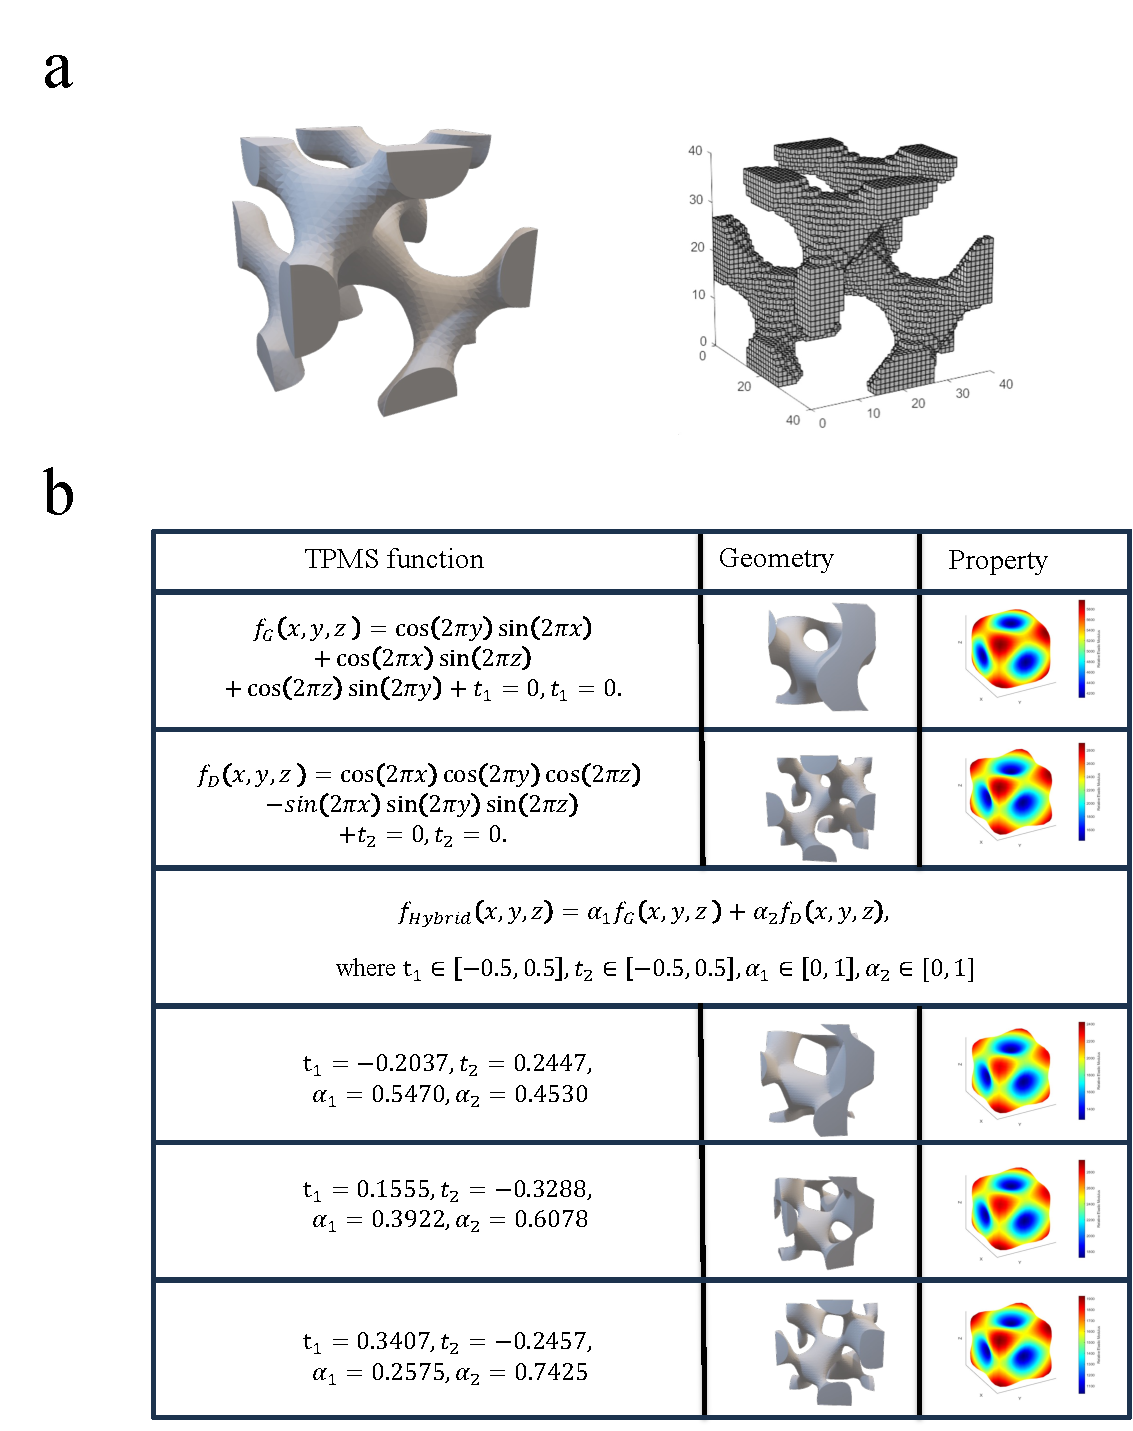
\includegraphics[width=1\linewidth]{figures/S1.pdf}
    \caption{Voxelization of a TPMS-based unit cell (\textbf{a}) and 3D visualization of effective elastic tensor (\textbf{b})}
    \label{fig:s1}
\end{figure}


\begin{figure}
    \centering
    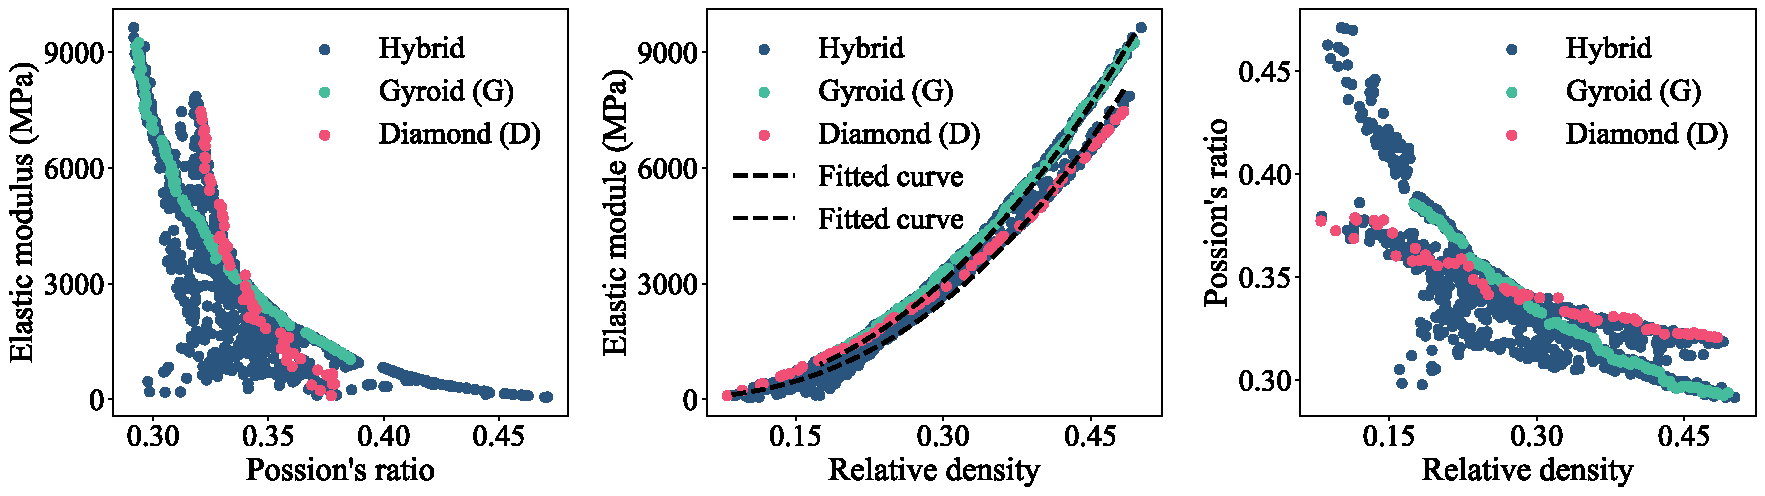
\includegraphics[width=1\linewidth]{figures/S2.pdf}
    \caption{The relationship between effective elastic modulus E, Possion's ration $v$ and relative density $\rho$.}
    \label{fig:s2}
\end{figure}

The voxelization of a TPMS-based unit cell and 3D visualization of effective elastic tensor obtianed by numerical homogenization method are shown in Fig S\ref{fig:s1}
In regions of low density, specifically when the relative density is below 0.2, the distribution of the elastic modulus is mixed. However, when the relative density exceeds 0.2, the relationship between the elastic modulus and relative density in hybrid structures bifurcates into two distinct categories. One trend aligns with the structure G, while the other aligns with the structure D. This division is illustrated by the fitted curves, depicted as black dashed lines (see Fig S\ref{fig:s2}). The corresponding fitted formulas are as follows:
\begin{equation}
    E_G = E_s\rho^{2.26}
\end{equation}
\begin{equation}
    E_D = E_s\rho^{2.42}
\end{equation}
where $E_s$ is the elastic modulus of Ti6Al4V.

The Ti6Al4V material has an elastic modulus of 46,532.9 MPa and a Poisson's ratio of 0.34. The plastic constitutive law is detailed in Table S\ref{tab:s1}\citep{Peng2023}.

\begin{table}
\centering
\caption{~Plastic constituent law of Ti6Al4V\citep{Peng2023}}
\begin{tabularx}{0.8\textwidth}{XX}
\toprule
Stress (MPa) & Plastic strain \\
\midrule
919.9167 & 0.000000000 \\
986.4167 & 0.010345953 \\
1041.8333 & 0.019444969 \\
1086.1667 & 0.028543986 \\
1119.4167 & 0.037643003 \\
1141.5833 & 0.046742019 \\
1139.3667 & 0.055841036 \\
1137.1500 & 0.064940052 \\
1131.6083 & 0.074039069 \\
1124.9583 & 0.083138085 \\
1116.0917 & 0.092237102 \\
1108.3333 & 0.101336118 \\
1075.0833 & 0.110435135 \\
1030.7500 & 0.119534152 \\
980.8750 & 0.128633168 \\
908.8333 & 0.137732185 \\
831.2500 & 0.146831201 \\
\bottomrule
\end{tabularx}
\label{tab:s1}
\end{table}

\section{Expected Improvement (EI)}
Expected Improvement (EI) is a widely used acquisition function in Bayesian optimization, which measures the expected improvement over the current best-known solution.

Assume we have observed a dataset $\mathcal{D}_n=\{x_{1:n},f_{1:n}\}$, where $f(x_i)$ represents the function value at point $x_i$. The current best-known value is $f^*_n=\max\{f_1,...,f_n\}$.

For a new point $x_{n+1}$ with function value $f_{n+1}$, the improvement is defined as:
\begin{equation}
    I(x_{n+1})=\max(f_{n+1}-f^*_n,0)
\end{equation}
This means improvement is only considered if $f_{n+1}$ exceeds the current best value $f^*_n$.

The Expected Improvement $\alpha_{\text{EI}}(x)$ is the expected value of the improvement $I_{\text{EI}}(x)$:
\begin{equation}
\alpha_{\text{EI}}(x)=\mathbb{E}[I_\text{EI}(x)|\mathcal{D}]=\mathbb{E}[\max(f_{n+1}-f^*_n,0)]
\end{equation}
Assuming the objective function $f(x)$ follows a Gaussian process, the predicted value $f_{N+1}$ at point $x$ follows a normal distribution $\mathcal{N}(\mu(x), \Sigma^2(x))$, where $\mu(x)$ and $\Sigma(x)$ are the posterior mean and standard deviation, respectively.

Thus, we have 
\begin{equation}
\alpha_{\text{EI}}(x)=\int_{-\infty}^{\infty}\max(f_{n+1}-f^*_n,0)\cdot p(f_{n+1}|x)df_{n+1}
\end{equation}
Since max($f_{n+1}-f^*_n, 0$) is zero when $f_{n+1}<f^*_n$, the integral can be simplified to:
\begin{equation}
  \alpha_{\text{EI}}(x)= \int_{f^*_n}^\infty(f_{n+1}-f^*_n)\cdot p(f_{n+1}|x)df_{n+1}
\end{equation}
\textbf{Reparametrization trick}

Let $z=\frac{f_{n+1}-\mu(x)}{\sigma(x)}$,  so $f_{n+1}=\mu(x)+\sigma(x)z$, and $p(f_{n+1}|x)$ becomes the standard normal density function $\phi(z)$. Therefore:

\begin{equation}
\begin{aligned}
  \alpha_{\text{EI}}(x)&=\int_{\frac{f^*_n-\mu(x)}{\sigma(x)}}^\infty(\mu(x)+\sigma(x)z -f^*_n)\cdot\phi(z)dz\\
    &=(\mu(x)-f^*_n)\int^\infty_{\frac{f^*_n-\mu(x)}{\sigma(x)}}\phi(z)dz + \sigma(x)\int^\infty_\frac{f_n^*-\mu(x)}{\sigma(x)}z\cdot \phi(z)dz
 \end{aligned}
\end{equation}
Using the properties of the standard normal distribution:
\begin{equation}
    \int_a^\infty z\cdot\phi(z)dz=-\phi(a)
\end{equation}
\begin{equation}
    \int_a^\infty\phi(z) dz = 1-\Phi(a)
\end{equation}
where $\phi (z)$ is the standard normal density function and $\Phi(z)$ is the standard normal cumulative distribution function.
Thus:
\begin{equation}
\begin{aligned}
  \alpha_{\text{EI}}(x)&=(\mu(x)-f^*_n)[1-\Phi(\frac{f^*_n-\mu(x)}{\Sigma(x)})]+\Sigma(x)\phi(\frac{f^*_n-\mu(x)}{\Sigma(x)}) \\
  &=(\mu(x)-f^*_n)\Phi(\frac{\mu(x)-f^*_n}{\Sigma(x)}) + \Sigma(x)\phi(\frac{\mu(x)-f^*_n}{\Sigma(x)}) \\
\end{aligned}
\end{equation}

\section{Toy Problem for Constraint-aware Active Learning}
The unconstrained objective function is defined as:
\begin{equation}
    f(x) = 0.001\cos(0.5x) + \frac{x}{30} + \sin(0.6x), \quad x \in [0, 17]
\end{equation}



The constraint function is given by:
\begin{equation}
c(x) = \frac{1}{1+e^{(x-8.5)}}, \quad x \in [0, 17]
\end{equation}

Consequently, the objective function incorporating the constraint can be expressed as:
\begin{equation}
f_c(x) = f(x) \cdot c(x), \quad x \in [0, 17]
\end{equation}
The maximum value of the unconstrained objective function, \( f(x) \), occurs at \( x = 13 \), whereas the maximum value of the constrained objective function, \( f_c(x) \), is located at \( x = 2.5 \). To model these functions, two Gaussian process regressions are employed. In Bayesian Global Optimization (BGO), an optimizer is used to search for a promising point \(\hat{x}\) by maximizing an infill criterion with respect to surrogate models, rather than relying on the 'true' objective functions. The constraint function applied to the objective function can similarly be applied to the infill criterion, or acquisition function.

The EI score and the constraint-aware EI score are derived from \(\alpha_{\text{EI}} = \mathbb{E}(I_{\text{EI}}(x))\) and \(\alpha_{\text{EI-C}} = \mathbb{E}(I_{\text{EI-C}}(x)) = \alpha_{\text{EI}}(x) \cdot c(x)\), respectively. The query point recommended by \(\alpha_{\text{EI-C}}\) achieve the optimal value in the constrained objective function \( f_c(x) \).

\section{Feature Normalization}

The structural parameters $\alpha_1$ and $\alpha_2$ of the TPMS are normalized before  being input to neural network, along with their geometric and property characteristics, such as relative density $\rho$, thickness $th$, pore diameter $d$, and effective modulus $E$. This normalization is achieved using the following equation:

\begin{equation}
(\hat{\cdot}) = 2 \times \frac{(\cdot) - \min(\cdot)}{\max(\cdot) - \min(\cdot)} - 1  
\end{equation}

\begin{table}
    \centering
        \caption{The hyper-parameters and architecture of TPMS-GAN($G_\phi^1$) }
    \begin{tabular}{|c|c|c|c|} \hline  
         Batch size&  23&  Learning rate& 0.0002\\ \hline  
         Epochs&  2000&  Latent space& 3\\ \hline  
         Input size&  4&  \textbf{Condition size}& 1\\ \hline
 $\lambda_{gp}$& 10& $\eta$&0.5\\\hline \hline  
 \multicolumn{4}{|c|}{Hidden layer of generator: 128, 256, 512, 1024}\\ \hline  
 \multicolumn{4}{|c|}{Hidden layers of discriminator: 1024, 512, 256, 128}\\ \hline  
 \multicolumn{4}{|c|}{Hidden layers of navigator: 1024, 512, 128}\\ \hline 
    \end{tabular}
    \label{tab:s2}
\end{table}

\begin{table}
    \centering
        \caption{The hyper-parameters and architecture of TPMS-GAN($G_\phi^2$) }
    \begin{tabular}{|c|c|c|c|} \hline  
         Batch size&  23&  Learning rate& 0.0002\\ \hline  
         Epochs&  2000&  Latent space& 3\\ \hline  
         Input size&  4&  \textbf{Condition size}& 3\\ \hline
 $\lambda_{gp}$& 10& $\eta$&0.5\\\hline \hline  
 \multicolumn{4}{|c|}{Hidden layer of generator: 128, 256, 512, 1024}\\ \hline  
 \multicolumn{4}{|c|}{Hidden layers of discriminator: 1024, 512, 256, 128}\\ \hline  
 \multicolumn{4}{|c|}{Hidden layers of navigator: 1024, 512, 128}\\ \hline 
    \end{tabular}
    \label{tab:s3}
\end{table}

\begin{table}
    \centering
        \caption{The hyper-parameters and architecture of ITPMS-GAN($IG_\psi$) }
    \begin{tabular}{|c|c|c|c|} \hline  
         Batch size&  23&  Learning rate& 0.0002\\ \hline  
         Epochs&  2000&  Input size & 4\\ \hline  
         Output size&  3& Hidden size & 1024, 512, 128\\ \hline   

    \end{tabular}
    \label{tab:s4}
\end{table}

\section{ML surrogte model}

For evaluating the effective elastic modulus \(E\) of the TPMS unit generated by TPMS-GAN (\(G_\phi^1\)) convinecely, a surrogate model was developed by comparing five machine learning models: linear regression, decision tree regression, random forest, support vector machine, and Gradient boost regression. Figure \ref{fig:s3} illustrates the mean and variance of the \(R^2\) values for these models, obtained through a 10-fold cross-validation method. Among the models evaluated, the random forest model demonstrated superior performance, achieving an \(R^2\) value of 0.976 with a variance of 0.0045.

\begin{figure}
    \centering
    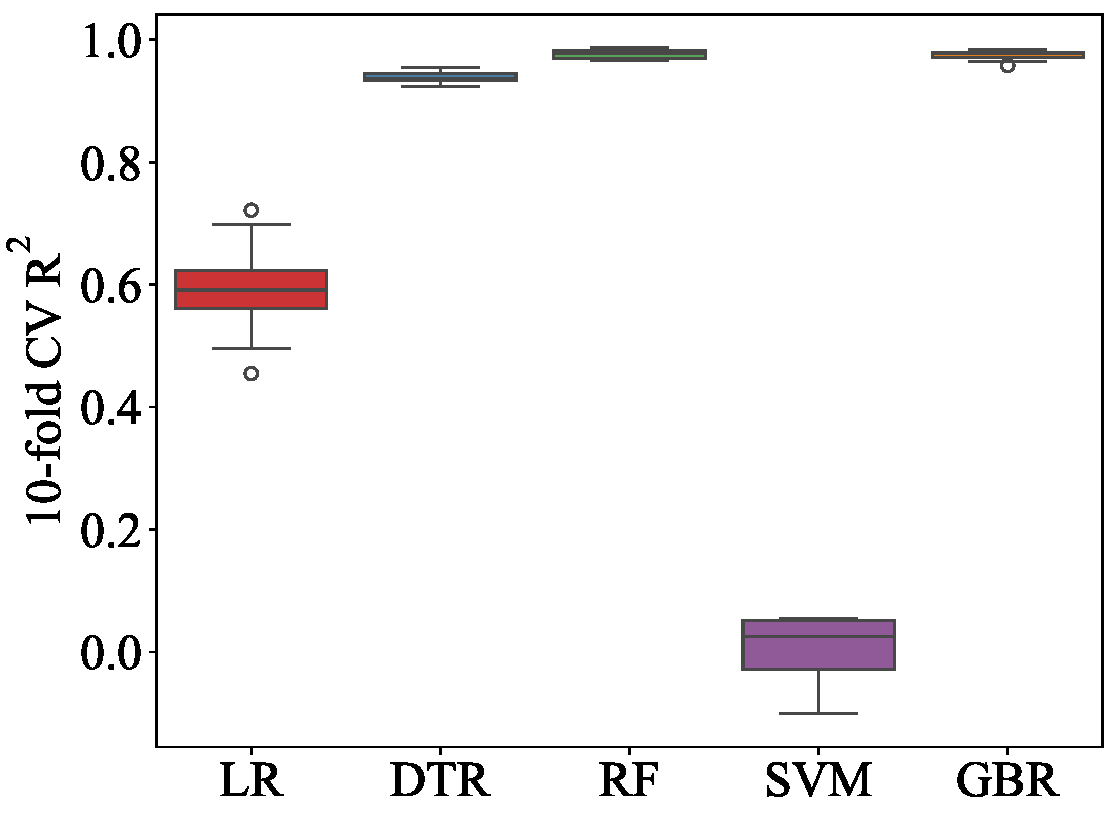
\includegraphics[width=0.5\linewidth]{figures/S3.pdf}
    \caption{Comparison of 10-fold $R^2$ of ML models}
    \label{fig:s3}
\end{figure}

\section{Computing Platform}
The neural network models training are performed in PyTorch on a laptop with 64 GB RAM and an Nvidia GeForce RTX 2060S GPU. The numerical homogenization method and COMSOL software are executed on a laptop with an Intel Core i7-10875H CPU featuring 8 cores.

%% If you have bibdatabase file and want bibtex to generate the
%% bibitems, please use
%%
\bibliographystyle{elsarticle-harv} 
\bibliography{refs}

%% else use the following coding to input the bibitems directly in the
%% TeX file.

% \begin{thebibliography}{00}

% %% \bibitem[Author(year)]{label}
% %% Text of bibliographic item

% \bibitem[ ()]{}

% \end{thebibliography}
\end{document}

\endinput
%%
%% End of file `elsarticle-template-harv.tex'.

